
\documentclass[a4paper,12pt]{article}
\usepackage{times}
\usepackage[francais]{babel}
\usepackage[utf8x]{inputenc}
\usepackage[T1]{fontenc}
\usepackage{amsmath}
\usepackage{amssymb}
\usepackage{graphicx}
\usepackage{pdfpages}
\usepackage{pdflscape}
\usepackage{listings}
\usepackage{longtable}
\usepackage{mathtools}
\lstset{literate=
{é}{{\'e}}1
{è}{{\`e}}1
{ê}{{\^e}}1
{à}{{\`a}}1
{â}{{\^a}}1
}
\lstset{language=C++,
basicstyle=\footnotesize,
keywordstyle=\footnotesize\color{blue},
otherkeywords={override,nullptr}
}
\definecolor{orange}{rgb}{0.8,0.4,0.0}
\definecolor{darkblue}{rgb}{0.0,0.0,0.6}
\definecolor{cyan}{rgb}{0.0,0.6,0.6}
\lstdefinelanguage{JSON}
{
basicstyle=\normalsize,
columns=fullflexible,
showstringspaces=false,
commentstyle=\color{gray}\upshape,
morestring=[b]",
morestring=[s]{>}{<},
morecomment=[s]{<?}{?>},
stringstyle=\color{orange},
identifierstyle=\color{darkblue},
keywordstyle=\color{blue},
morekeywords={string,number,array,object}% list your attributes here
}

\sloppy

\setlength{\topmargin}{0cm}
\setlength{\headsep}{0.in}
\setlength{\headheight}{0.in}
\setlength{\evensidemargin}{0cm}
\setlength{\oddsidemargin}{-1cm}
\textwidth 18cm
\textheight 25cm

\begin{document}

    \thispagestyle{empty}

    \begin{titlepage}

        \vspace*{2cm}

        \begin{center}\textbf{\Huge Projet Logiciel Transversal}\end{center}{\Large \par}

        \begin{center}\textbf{\large Anand Candassamy \& Paul Estano}\end{center}{\large \par}

        \vspace{2cm}

        \clearpage

        {\small
        \tableofcontents
        }

    \end{titlepage}

    \clearpage
    \section{Présentation Générale}

    \subsection{Archétype}
	    Notre jeu s'inspirera principalement du jeu \emph{Pokemon Donjon Mystère}. En effet, nous avons prévu de conserver le mécanisme des combats et de donjon de ce jeu.
	    \\Dans notre logiciel l'utilisateur incarnera un pokemon dans les salles d'un donjon qui contiennent chacune des pokemons qui peuvent l'"agresser". Le nombre de pokemons dans une salle évolue en fonction de l'avancement du joueur dans le jeu. 
	    \\Pour simplifier le jeu nous abandonnons également d'évolution des pokemons.

    \subsection{Règles du jeu}
	  Le donjon contient un nombre fini de salles et le joueur gagne lorsqu'il sort de la dernière salle du donjon.
	  Un donjon a 10 salles, le pattern de chaque étage n'est pas tiré aléatoirement. Le joueur a la possibilité d'accéder à des étages bonus, dîtes arène de combat où il pourra se battre contre un autre joueur en ligne.
	   \\Le joueur est provoqué en duel automatiquement par les pokemons qui sont autour de lui. Il faut qu'il tue l'IA ou le joueur adverse pour activer la case de l'esaclier qui leur permet de passer à l'étage suivant.
\\Les combats fonctionnent en tour par tour. A chaque tour, l'utilisateur peut effectuer une action :
\begin{itemize}
    \item attaquer avec une compétence
    \item soigner le pokemon
    \item se déplacer d'une case
\end{itemize}
\clearpage
    \subsection{Ressources}
    \begin{figure}[ht]
    \begin{center}
        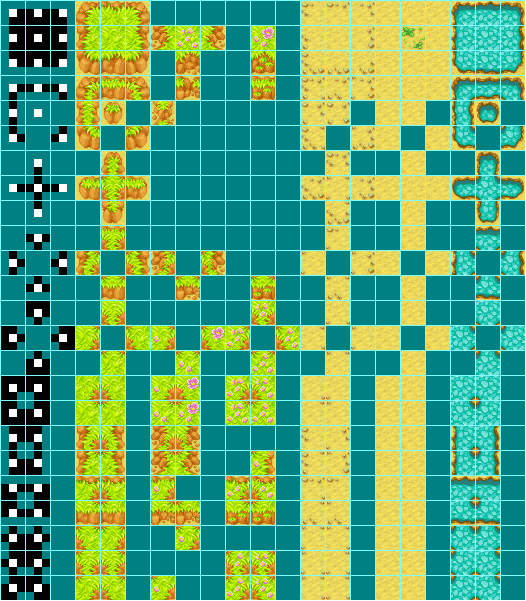
\includegraphics[width=0.8\textwidth]{tilemap.png}
    \end{center}
    \caption{Tileset utilisé pour construire un monde}
    \end{figure}
    
    \begin{figure}[ht]
    \begin{center}
        
\includegraphics[width=0.8\textwidth]{pokemonLatex.png}
    \end{center}
    \caption{Tileset utilisé pour les pokémons}
    \end{figure}



    \clearpage
    \section{Description et conception des états}
    
    \subsection{Description des états}
    Un état du jeu est formé d'une carte qui est statique au cours du temps et d'une liste de joueurs dont l'état varie au cours du jeu.
    
     \subsubsection{État de la carte}
     
     La carte est un élément fixe de l'état du jeu. Il se décompose en plusieurs cases.
    
     Les cases se distinguent en 3 parties : \begin{itemize}
    \item les murs, qui ne sont pas franchissables par les éléments mobiles.
    \item les cases "conteneurs", elles peuvent être vide ou occupé par un seul élément mobile.
    \item les cases escaliers, il en existe un seul par étage, qui permet d'aller au niveau suivant du labyrinthe.
    
    \end{itemize}

    \subsubsection{État des joueurs}
    Un pokemon est soit contrôlé par un joueur soit contrôlé par une Intelligence Artificielle (I.A), il possède une position, un nombre de points de vie à l'état t, un nom et un ensemble de statistiques qui lui sont attribués en début de partie. Le pokemon est considéré comme étant "mort" si son nombre de points de vie atteint 0.
    
    \subsubsection{État général}
    A l’ensemble des éléments statiques et mobiles, nous rajoutons les propriétés suivantes :
    — Époque : représente « l’heure » correspondant à l’état, ie c’est le nombre de « tour » passés
    globale depuis le depuis de la partie.

    
    Ces statistiques correspondent aux attaques qu'il peut utiliser, à son nombre de point de vie en début de partie et son type (Salameche, Bulbizarre, Carapuce).
    \subsection{Conception Logiciel}
    Le package état peut se diviser en trois sous-partie:\begin{itemize}
        \item Une partie gérant les personnages, en bleu
        \item Une partie gérant l'environnement, en rouge
        \item Une classe représentant l'état global du jeu, en vert
    \end{itemize}
    
     La classe \emph{Player} contient l'ensemble des éléments permettant de caractériser l'état d'un joueur. Chaque joueur est lié à un pokemon par une relation de composition : un pokemon ne peut pas exister sans joueur. Dans le cas où le pokemon est contrôlé par l'IA, l'IA est considérée comme un joueur et contrôle donc son pokemon.
     
    Pour notre implémentation du jeu, nous avons prévu d'utiliser que les trois pokémon suivant : \begin{itemize}
        \item Carapuce
        \item Salamèche
        \item Bulbizarre
    \end{itemize}
    Le constructeur respectif de chacun de ces trois pokemons héritent de la classe Pokemon. Nous avons mis en place un identifiant pour chaque pokemon, ce qui permet d'avoir plusieurs pokemon construit à partir de la même classe.
    
    Chaque pokemon possède une orientation (\emph{SOUTH, NORTH, WEST ou EST}), et un nombre de points de vie maximum qui dépend de son type (\emph{SALAMECHE, CARAPUCE, BULBIZARRE}) .
    
    La partie environnement est calqué sur le modèle proposé par les fichiers exportés par le logiciel \emph{Tiled Map Editor} au format JSON. Les objets les plus consommateurs en mémoire tels les \emph{data} dans la classe \emph{Layer} sont par ailleurs stockés dans le tas pour éviter les copies entre les différentes classes.
    
     L'état global contient un pointeur vers l'état de l'environnement et et une liste de pointeur de contenant l'état des différents joueurs de la partie. Un booléen permettant de détecter la fin du jeu a également été ajouté. 
     
     On utilise le pattern \emph{Observer} pour notifier les éléments dépendant de l'état lorsque celui-ci change. La classe \emph{State} hérite de la classe \emph{Observable} qui contient une liste d'objets héritant de la classe abstraite \emph{Observer}. Lorsque la classe \emph{State} subit un changement, l'utilisateur utilise la méthode \emph{notifyObservers()} pour notifier ses observers avec l'évènement correspondant au changement appliqué.
     Il existe 2 types d'\emph{Event}:
\begin{itemize}
\item Les \emph{TAB\_EVENT} qui représente un changement d'état lié à la position des pokemons sur la carte (absent si mort, changement de position , changement d'orientation)
\item Les \emph{STATE\_EVENT} qui correspondent à des changement liés à l'environnement (changement de niveau) ou à des changements liéés aux statistiques de la partie
\end{itemize}
     d{itemie}
  Afin d'éviter des problèmes techniques dans notre implémentation, nous avons mis en place des fonctions afin de capturer les exceptions rencontrées lors de l'exécution, principalement dans la classe qui charge les données de la carte. De plus nous avons utilisé des entiers non signés afin que les attributs des pokemons ne prennent jamais de valeurs négatives.
    
    \begin{landscape}
    \begin{figure}[p]
    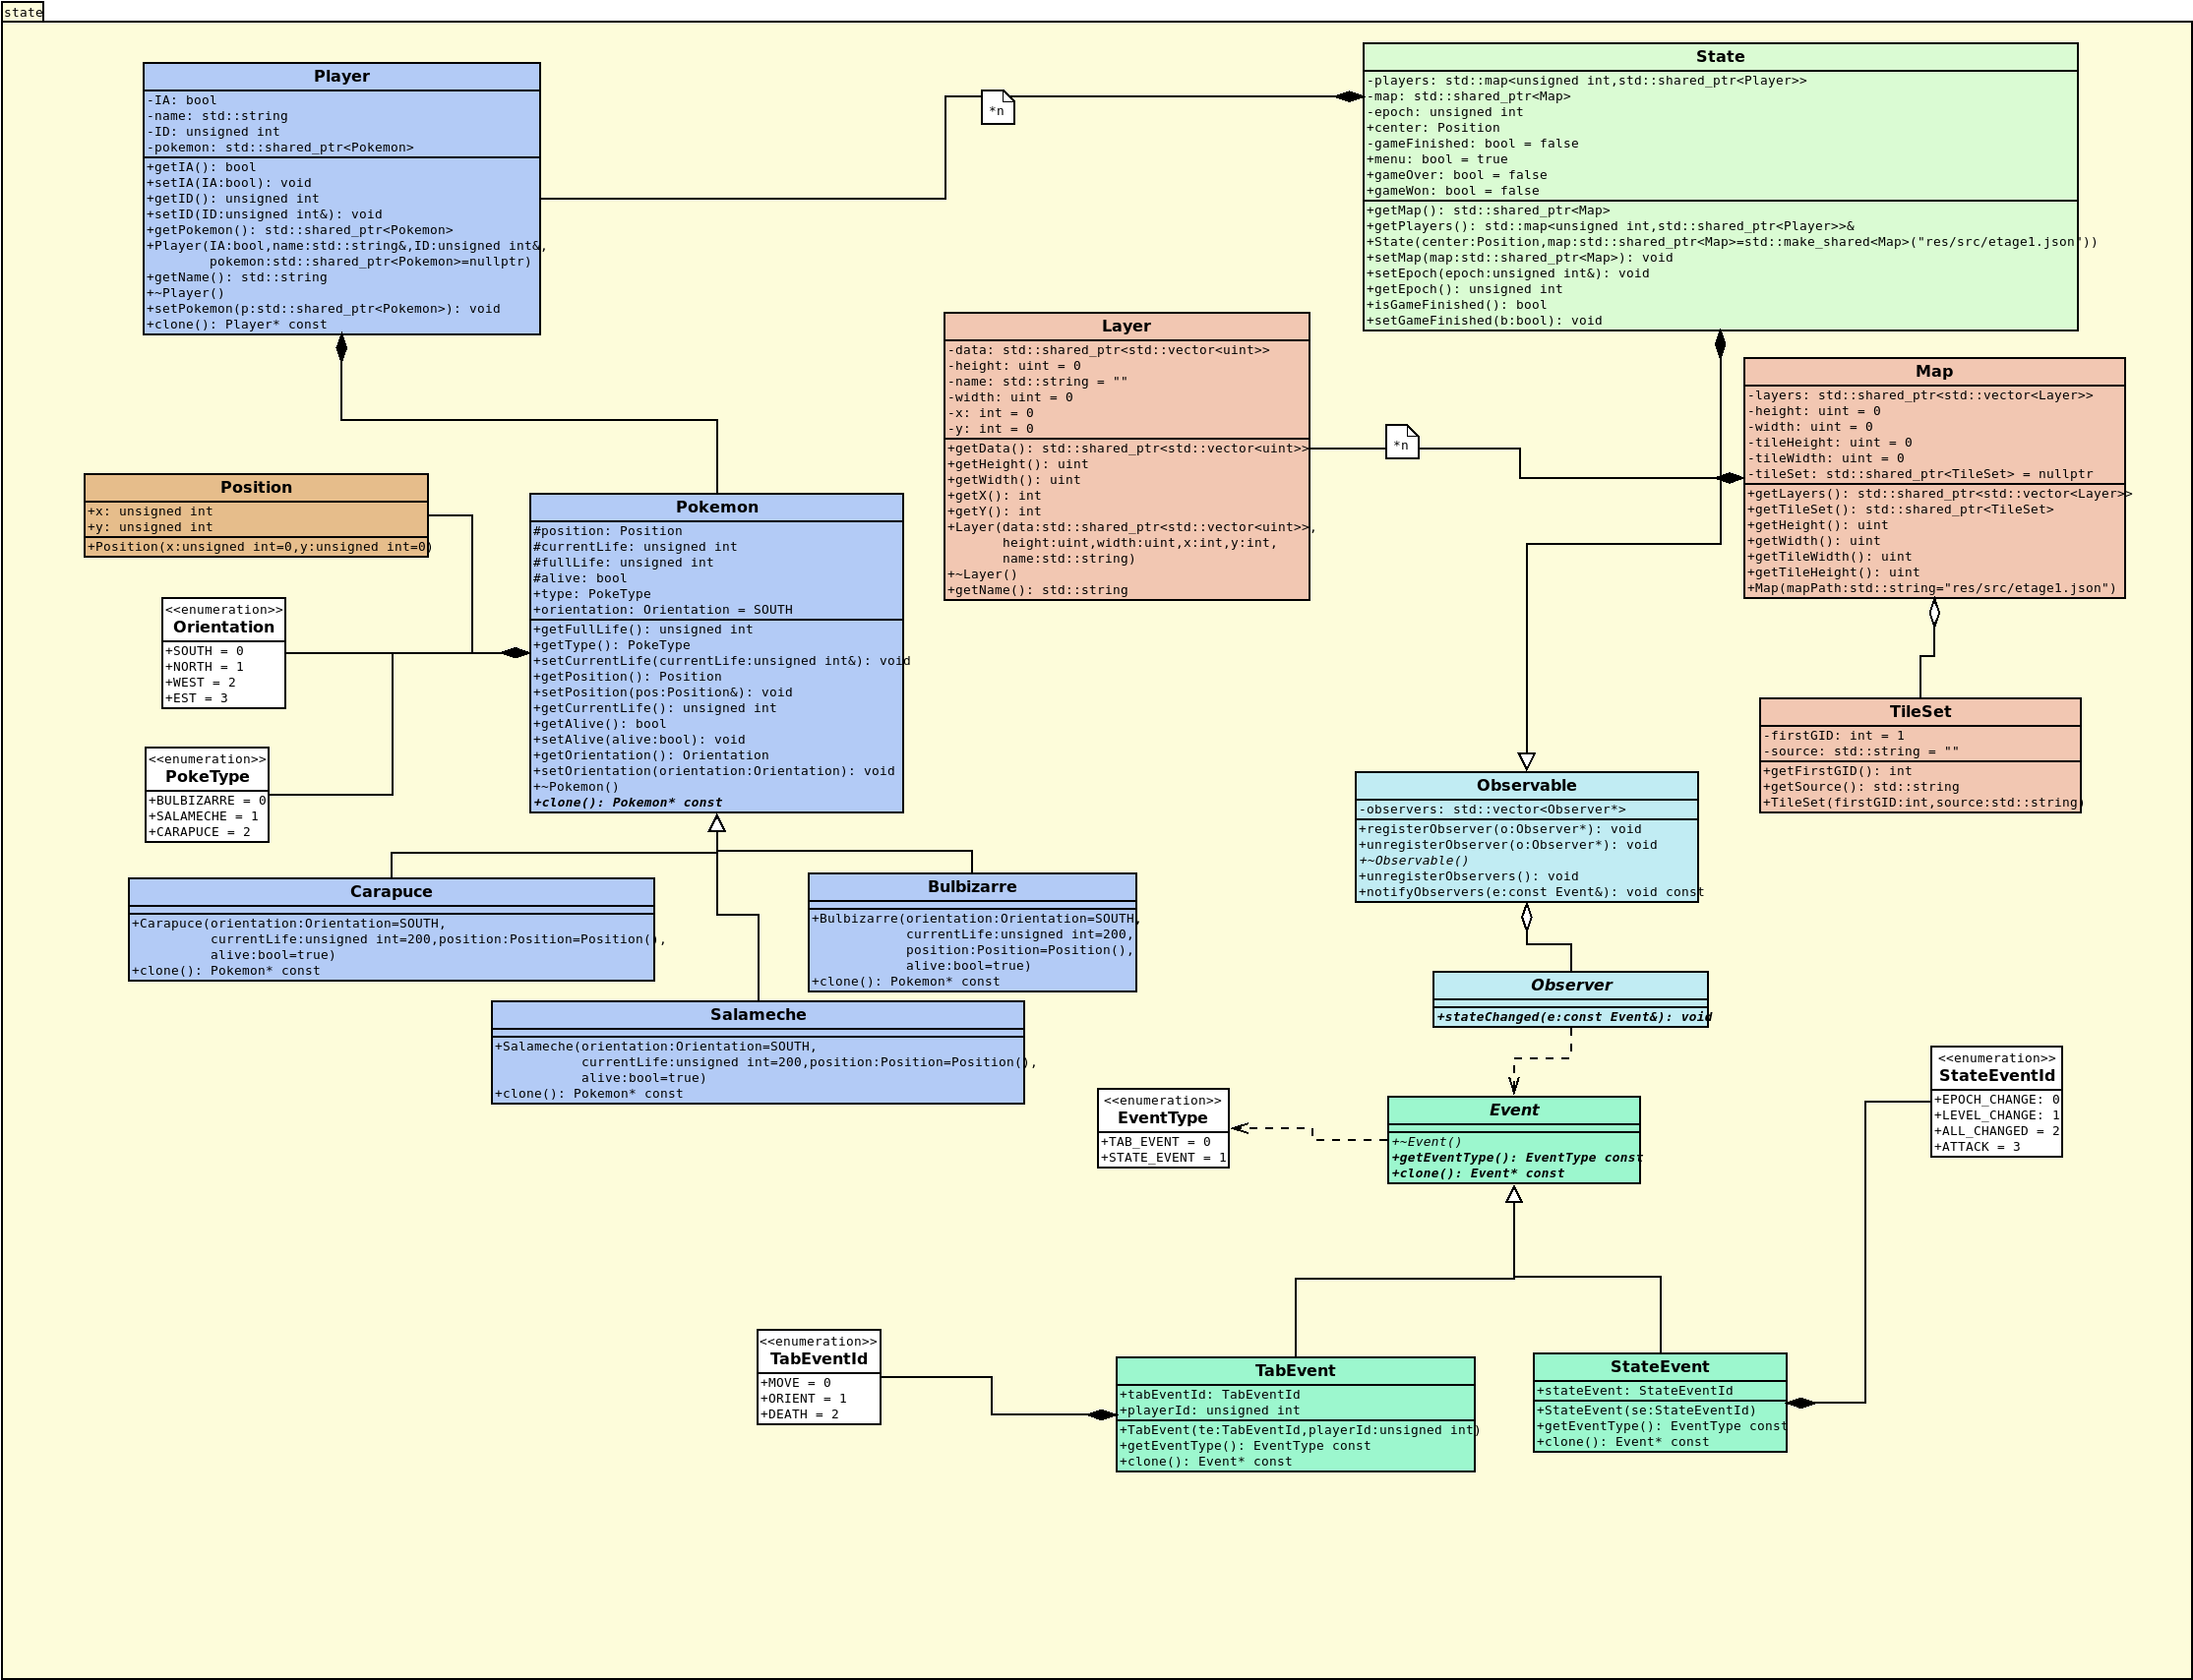
\includegraphics[width=0.8\paperheight]{state.png}
    \caption{\label{uml:state}Diagramme des classes d'état.}
    \end{figure}
    \end{landscape}
    \clearpage
    
    
    \section{Rendu: Stratégie et Conception}

    \subsection{Stratégie de rendu d'un état}
    
Notre stratégie de rendu d'un état se base sur l'utilisation de l'interface SFML qui s'appuie sur OpenGL afin de générer un rendu en 2D. Nous avons utiliser les fonctions de SFML afin de charger dans le processeur, la liste des éléments à afficher par le processeur graphique. 
    
Nous avons découpé notre affichage graphique sur deux niveaux, la carte avec les éléments décoratifs (mur, sol, escalier) et les éléments mobiles à savoir les pokemons (Carapuce, Salamèche, Bulbizarre) qui se superposent sur la couche précédente. On transmet l'état du jeu ainsi que les textures de toute la carte avec leurs coordonnées et la texture des pokemons avec leurs coordonnées et leur orientation à afficher.
        
La carte étant très grande, nous l'avons entièrement chargé dans la mémoire pour l'affichage et on a créé une vue (un zoom) centrée sur le pokemon du joueur qui évolue sur la carte, car le but du jeu reste avant tout d'évoluer dans un labyrinthe.
     
Lorsque qu'un changement d'état se produit, la vue est modifiée en fonction du changement appliqué à l'état. Si le changement modifie uniquement la position des pokemons, seule le rendu des pokemons est mis à jour, si ce changement s'applique à l'environnement l'ensemble du rendu de la carte est mis à jour. Lorsque l'ensemble de l'état est modifié le rendu de l'état est entièrement mis à jour. Dans le cas où le jeu est fini la fenêtre est automatiquement fermée.

Nous avons rajouté sur la scène finale, certains attributs des pokemons (point de vie actuelle et id des pokemon) en haut à gauche. 
        
Pour simplifier au mieux notre logiciel, nous n'avons pas inclus les animations de déplacements lorsque le pokemon évolue d'une case à l'autre ainsi que les animations d'attaques quand un pokemon lance une compétence sur un autre.


    \subsection{Conception logiciel}
Pour afficher un état on crée une scène qui génère un ensemble de pointeurs sur des objets graphiques de types \emph{LayerRender} pour la carte.
Pour les Pokemon, on instancie un \emph{Sprite} par Pokemon. Ce \emph{Sprite} contient à la fois les coordonnées du Pokemon sur la fenêtre et sa position sur le Tileset utilisé. Puis, on utilise la méthode \emph{Scene::draw()} pour déclencher l'ouverture de la fenêtre et l'affichage de l'état.
Il est à noter que l'état contient d'ores et déjà toutes les informations nécessaires à l'affichage de la carte. En effet, à la création de l'état celui-ci parse un fichier JSON (ici \emph{map.json})contenant toutes les informations nécessaires à l'affichage de la carte.

 classe \emph{Scene} est un des \emph{Observer} de \emph{State}. Ainsi, lorsque l'état subit un changement, \emph{Scene} est notifié et met à jour le rendu en fonction du type d'évènement qui lui est transmis:
\begin{itemize}
\item Si un \emph{TAB\_EVENT} (correspondant à changement d'état pour l'un des joueurs) la méthode \emph{updatePlayers()} responsable de la mise à jour du rendu des pokemon est appelée.
\item Si un \emph{STATE\_EVENT} (correspondant changement d'état lié à l'environnement ou à la partie) les méthodes \emph{updatePlayers()} et \emph{updateMap()}.
\end{itemize}
Par ailleurs, les points de vie de chacun des pokemon sont, pour le moment, affichés et mis à jour en temps réel à l'intérieur de la méthode \emph{draw()} de la classe \emph{Scene}.

Chaque objet \emph{LayerRender} parcourt l'ensemble des tuiles d'un étage de la carte, détecte la position de la tuile sur la ressource graphique (i.e : l'image du tileset) et calcule sa position sur la fenêtre. Pour optimiser les performances seule l'image du tileset est chargée dans une \emph{Texture}, l'objet \emph{LayerRender} conserve seulement la position de chaque tuile de la carte sur cette texture.
Les pokemons sont chacun rendus à l'intérieur d'un \emph{Sprite}.
Lorsqu'un mouvement de l'un des pokemons est détecté le la classe scène met à jour l'affichage de l'ensemble des pokemons.

    \begin{landscape}
    \begin{figure}[p]
    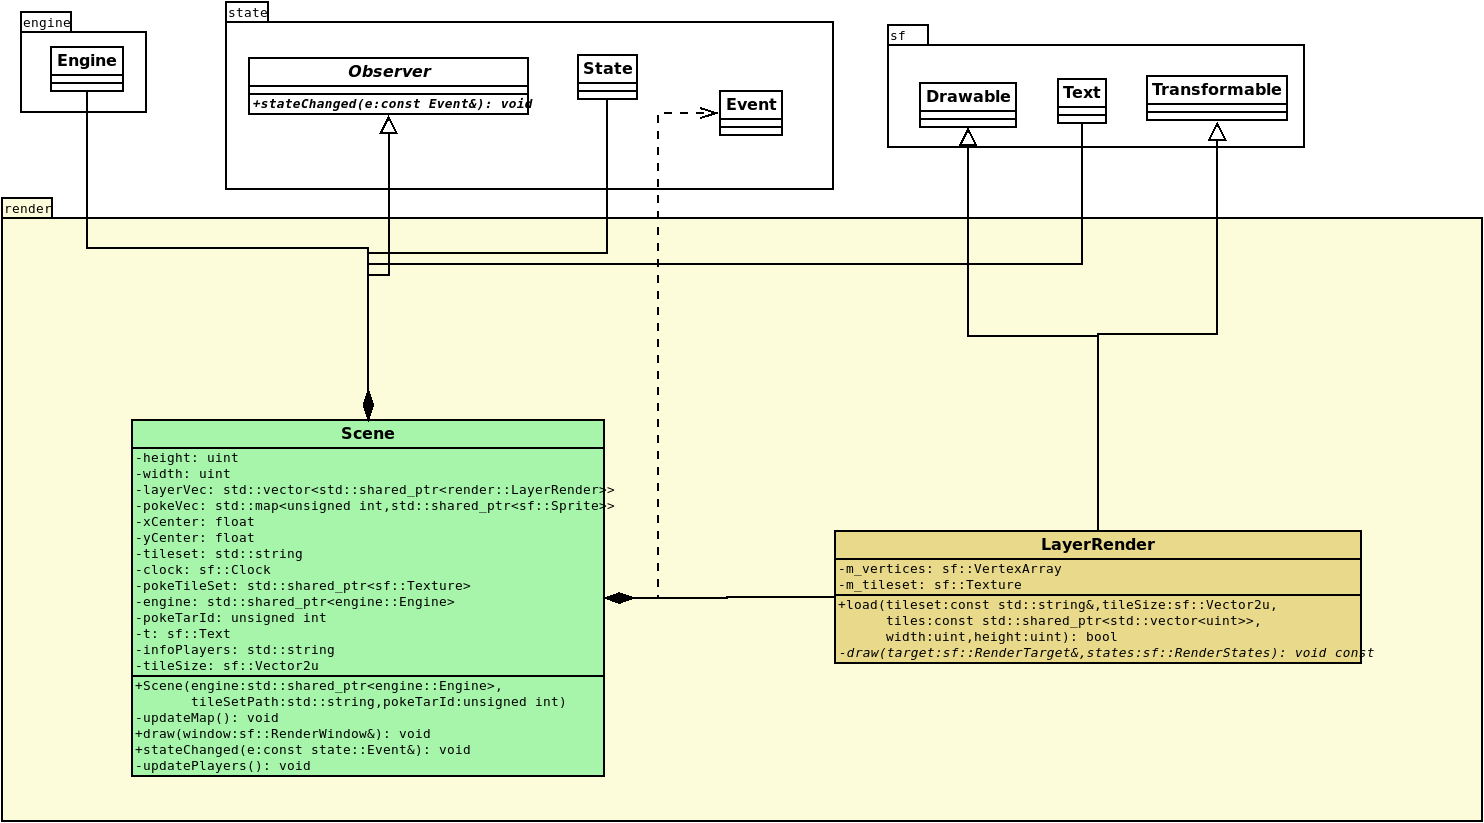
\includegraphics[width=0.9\paperheight]{render.png}
    \caption{\label{uml:render}Diagramme des classes de rendu.}
    \end{figure}
    \end{landscape}

    \clearpage
    \section{Règles de changement d'états et moteur de jeu}

    \subsection{Règles}
    
    Les changements d'états sont liés aux commandes exécutées par le moteur.
    Les commandes extérieures sont : 
    \begin{itemize}
        \item Commande de déplacement
        \item Commande d'attaque
        \item Commande de soin
    \end{itemize}
    
    Une fois qu'une commande extérieure de la part du joueur et de l'IA ont été exécutés (joueur puis IA), on passe au tour suivant.
    
    \subsection{Changements autonomes}
    
    Les changements autonomes interviennent à la fin de chaque changement d'état lié à une commande extérieure et s'exécutent dans l'ordre suivant : 
    \begin{enumerate}
        \item Si le joueur est mort, on affiche "GAME OVER"
        \item Si l'IA est morte, on active la case escalier pour passer à l'étage suivante
        \item On met à jour les statistiques (point de vie) de l'IA et du joueur en fonction des règles d'attaque et de soin.
        \item On applique les règles de déplacement du joueur et de l'IA. 
        \item Si le joueur est sur la case d'escalier, on vérifie s'il est autoriser à passer au niveau suivant.
\item Si le joueur a gagné on affiche "GAME WON"
    \end{enumerate}
    
    
    
    
    


    \clearpage
    \subsection{Conception logiciel}
On utilise ici le pattern \emph{Command}: un ensemble d'utilisateur peut ajouter des "commandes" à l'objet \emph{Engine} puis lui demander de les exécuter à l'aide de la méthode \emph{runCommands()}.

Les commandes hérite de la classe abstraite \emph{Command} contient une méthode \emph{execute()} virtual pure qui est appelée par le moteur lorsqu'un utilisateur appelle la méthode \emph{runCommands()}. Cette méthode applique en fait directement des changements à l'objet \emph{State} conservé par la classe \emph{Engine}.

On a  implémenté, pour le moment, 3 types de commande:
\begin{itemize}
\item \emph{MoveCommand} qui correspond à un changement de position d'un des pokemon
\item \emph{AttackCommand} qui correspond à l'attaque d'un pokemon
\item \emph{HealCommand} qui est déclenché lorsqu'un joueur veut soigner son pokemon 
\end{itemize}

Les trois commandes \emph{MoveCommand}, \emph{AttackCommand} et \emph{HeakCommand} sont déclenchés sur un évènement de lecture de clavier, plus précisement sur un évènement d'appui sur une touche de clavier pour plus de fluidité lors des déplacements dans le parcours du labyrinthe.

La commande \emph{MoveCommand} met à jour la position ou l'orientation du pokemon sur la map.

Les commandes \emph{AttackCommand} et \emph{HeakCommand} agissent sur l'état des pokemon et sur le rendu de la scène en gardant à jour les points de vie actuels affichés en haut à gauche de la scène.

Par ailleurs, le changement de niveau étant provoqué par un déplacement sur la case escalier après qu'un joueur (non IA) ait éliminé tous ses ennemis; cet évènement est entièrement géré et intégré à la commande \emph{MoveCommand}.

Lors de l'exécution de chaque commande, on crée un objet associé à la commande qui permet de sauvegarder des données importante de l'état du jeu comme la vie, la position et l'orientation d'un pokémon. 
\\Ces données sont stockées dans des objets de type \emph{PreviousState} et eux même stockés dans une \emph{stack}, ce qui permet d'annuler les commandes exécutées précédemment en dépilant un à un les éléments contenus dans cette \emph{stack} grâce à la méthode \emph{undoCommands()}.

    \begin{landscape}
    \begin{figure}[p]
    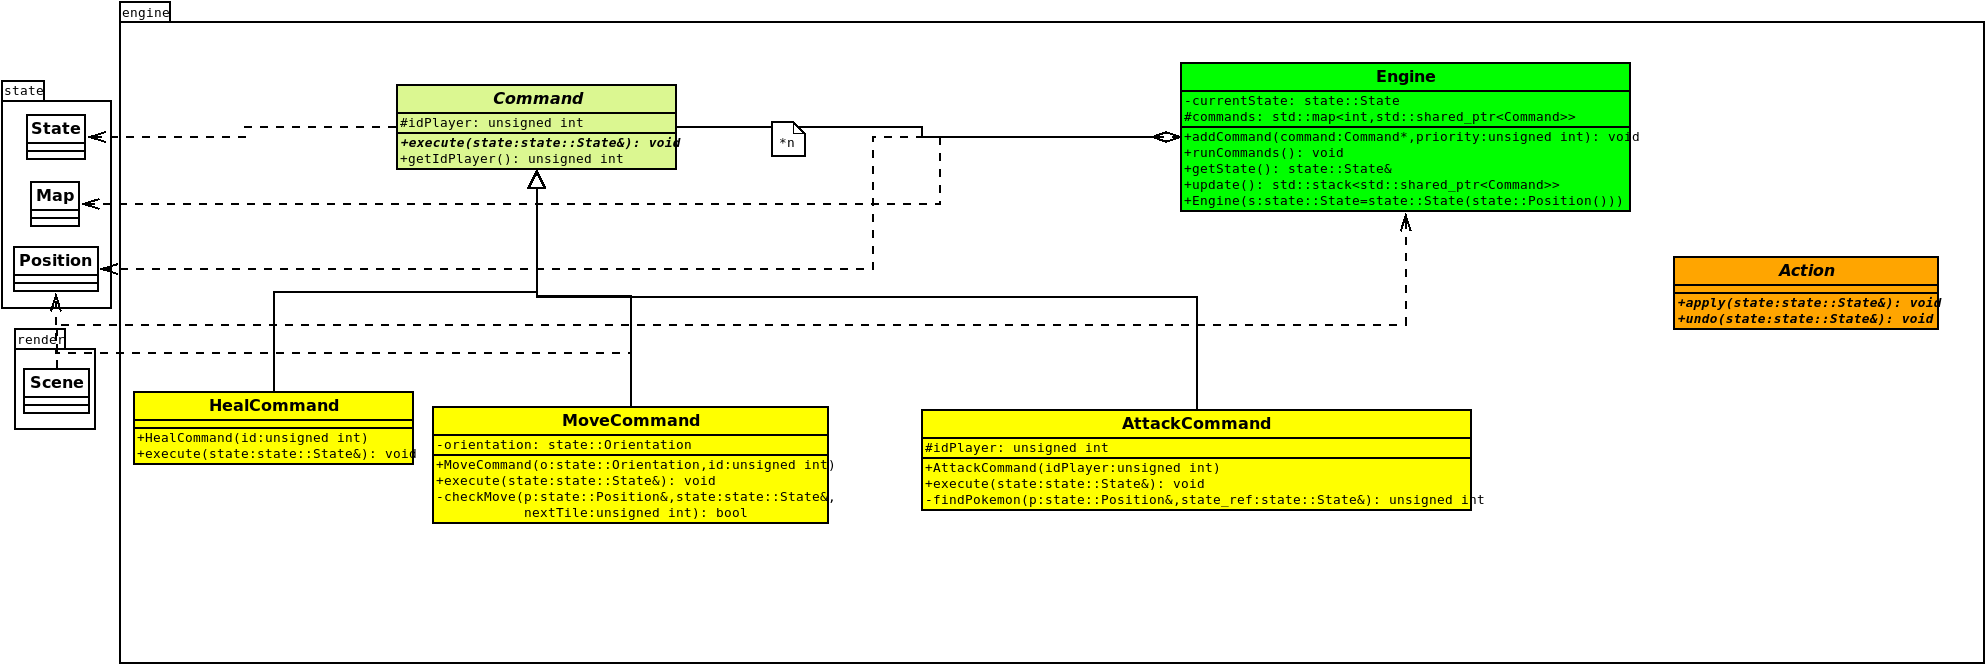
\includegraphics[width=0.9\paperheight]{engine.png}
    \caption{\label{uml:engine}Diagramme des classes de moteur de jeu.}
    \end{figure}
    \end{landscape}


    \section{Intelligence Artificielle}

    \subsection{Stratégies}
    \subsubsection{Intelligence aléatoire}
    
    Le stratégie de l'AI aléatoire est de se déplacer de manière aléatoire sur la map, lors qu'il rencontre un ennemi, il peut alors combattre et lorsque ses pv tombent bas, il se soigne.
    
    \subsubsection{Intelligence basé sur les heuristiques}
    
    Nous avons ajouté des heuristiques aux pokémons ennemies afin qu'il puisse battre le pokémon du joueur :\begin{enumerate}
        \item Si le pokémon a un nombre de points de vie supérieur à celui de son adversaire, il l'attaque si il est en face de lui. 
\item Si le pokemon a un nombre de points de vie supérieure ou égale à celui de son adversaire et qu'il est à distance de celui-ci, il se rapproche.
        \item Si le pokémon a un nombre de points de vie trop faible pour gagner le combat, il tentera de fuir son adversaire si celui-ci peut l'attaquer.
         \item Si le pokémon ne risque pas de perdre des points de vie suite à une attaque ennemie et qu'il lui en manque, il tentera de se soigner.
    \end{enumerate}
    Et finalement pour que le pokémon ennemi se rapproche de celui du joueur, nous avons utilisé l'algorithme A* qui est un algorithme de recherche de chemin dans une graphe (ici notre carte).
    Nous avons notamment utilisé le code disponible ici : \textcolor{blue}{\underline{ https://github.com/daancode/a-star}}
    
    \subsubsection{Intelligence avancée}
        Nous proposons en dernier lieu une intelligence avancée basée sur l'algorithme minmax à deux joueurs. Dans notre implémentation, l'IA avancée va explorer toutes les issues possibles et va tenter de maximiser ses chances de victoire face au joueur. Pour cela, nous avons implémenté une fonction de coût : 
        \begin{equation}
        cost  =  Life_{AI} -   D_{AI/Player} - Life_{Player}
        \end{equation}        \\Cette fonction exprime trois comportements de l'IA avancée :\begin{enumerate}
            \item le fait de se déplacer quand il ne voit pas d'ennemi autour, caractérisé par la distance entre l'IA et le Joueur.
            \item le fait d'attaquer l'ennemi lorsqu'il est en position de force, qui résulte de la différence de points de vie entre l'IA et le Joueur.
            \item le fait de s'enfuir et de se soigner lorsqu'il est en position de faiblesse qui résulte lui aussi de la différence de points de vie entre l'IA et le Joueur.
        \end{enumerate}
        
        Ainsi à chaque tour, l'IA avancée va choisir le coup optimal parmi l'ensemble des actions qu'il peut effectuer et qui va maximiser ses chances de gagner au tour suivant grâce à cette fonction de coût où l'un des trois comportements va être mis en avant par rapport aux deux autres. Pour cela, l'algorithme va parcourir l'ensemble des issues possibles à chaque tour. Pour effectuer cette tâche, on a choisi de dupliquer la partie de l'état nécessaire au bon fonctionnement de l'algorithme (état des joueurs et des pokemons) à chaque noeud de l'arbre de recherche.\\
        Pour ce qui est du déplacement sur la carte, nous avons gardé le même algorithme que celui de l'heuristique, à savoir le A *, afin que l'IA puisse se diriger et s'orienter vers le joueur sur la carte de façon optimum.
    
    
    \clearpage
    \subsection{Conception logiciel}
    
    Le diagramme des classes d'AI est affiché ci-dessous
    
    \emph{Classes AI}. Les classes filles de la classe AI implémente 3 stratégie d'IA suivi par le pokemon adverse :\begin{enumerate}
      
\item RandomAI : Intelligence Artificielle aléatoire
\item HeuristicAI :  Intelligence Artificielle Heuristique
\item DeeoAI : Intelligence Artificielle avancée
    \end{enumerate}
    \textbf{AStar Generator} :
    \\Malheureusement, le code provenant d'un projet extérieur, nous n'avons pas pu intégrer les classes du AStar dans notre fichier \emph{ai.dia}.
    Pour utiliser le générateur on doit tout d'abord les fournir une version "alléger" de l'environnement ( i.e. de la classe \emph{Map} ) contenant seulement les obstacles de la carte.
   \\\textbf{AIUtils} :
   \\Nous avons également séparé plusieurs méthodes utilitaires consommées par HeuristicAI (et à l'avenir par DeepAI) dans une classe \emph{AIUtils}. Ses méthodes étant indépendantes, elles sont déclarées comme \emph{static} ce qui permet de les utiliser sans instancier d'objet superflus. 
   La méthode flee permet notamment de calculer le meilleurs déplacement possible pour fuir un adversaire.
    \\\textbf{DeepAI} :
	\\C'est une IA basée sur la résolution de problème à état finis. On utilise l'algorithme de parcours d'abres minmax. Ici on a un pokemon contre un autre.  Les critères de "jugement" de l'IA sont :
    \begin{itemize}
    \item     Sa vie qu'elle veut  maximiser
\item La vide de l'ennemi  qu'elle veut minimiser
\item Sa distance à l'ennemi qu'elle veut minimiser
    \end{itemize}
    Malheureusement, l'environnement étant relativement grand il est impossible pour l'IA de parcourir l'arbre de recherche en profondeur à chaque coup. En effet chaque noeud de l'arbre possède 4 branches ( fuir, se soigner, attaquer, se rapprocher) et la carte, bien que possédant des murs et des obstacles, contient 25x25 = 625 cases. Ainsi, on comprend qu'il est impossible de parcourir l'ensemble de l'arbre dans un temps acceptable. 
    Dans la pratique, l'algorithme parcourt au maximum 4 niveaux de l'arbre. Malheureusement, cela ne semble pas suffisant pour obtenir une intelligence plus performante que l'IA Heuristique. 
    Pour améliorer la performance de l'algorithme nous pourrions mettre en place des conditions pour le parcours des noeuds de l'arbre de recherche pour ainsi éviter le parcours de noeuds inutiles (algorithme alpha bêta). 

    \begin{landscape}
    \begin{figure}[p]
    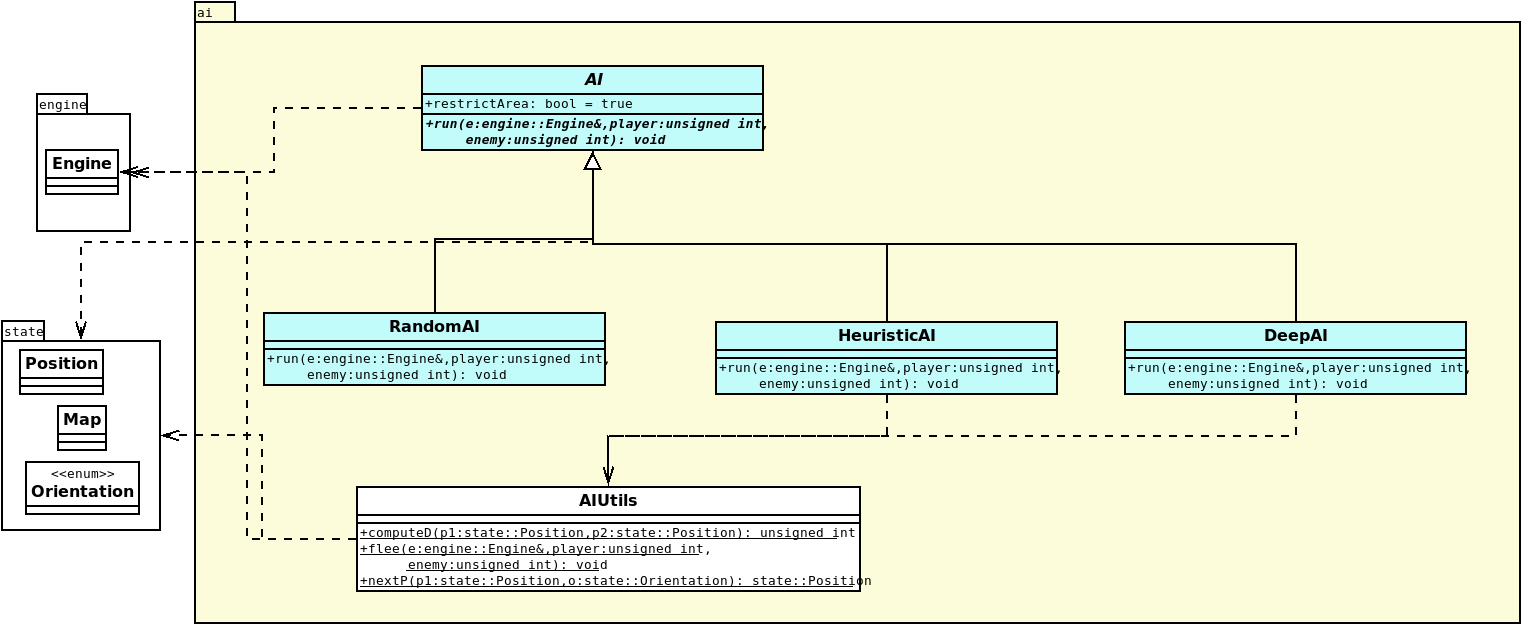
\includegraphics[width=0.9\paperheight]{ai.png}
    \caption{\label{uml:ai}Diagramme des classes d'intelligence artificielle.}
    \end{figure}
    \end{landscape}


    \section{Modularisation}
    \label{sec:module}

    \subsection{Organisation des modules}
	On veut ici lancer le moteur et le rendu dans deux threads différents. Le thread principal sera celui du rendu (contrainte matérielle) et le secondaire celui du moteur. Deux types de données transitent entre le moteur et le rendu : 
\begin{itemize}
\item Les commandes, qui transistent du rendu vers le moteur
\item Les évènements notifiant le rendu d'un changement d'état
\end{itemize}
\subsubsection{Commandes}
    Les commandes peuvent arriver à tout moment et l'ajout d'une commande à la map contenant les commandes lors d'une mise à jour de l'état de jeu pourrait engendrer des conflits. Pour palier à ce problème, on utilise un double buffer : lorsqu'une mise à jour de l'état a lieu, on vide la map dans un buffer, que l'on va ensuite utiliser pour exécuter l'ensemble des commandes. Pour empêcher l'ajout d'une commande dans la map lors de la copie dans le buffer, on utilise un mutex (\emph{commands\_mutex}) qui bloque l'exécution de la méthode \emph{addCommand} pendant toute la durée de la copie. Le temps de copie restant négligeable, l'utilisateur peut ajouter des commandes aussi rapidement qu'il le souhaite presque sans aucune latence.
\subsubsection{Notifications de rendu}   
    Lors d'une mise à jour, l'état notifie le rendu par le biais d'\emph{events}. Pour le moment, le traitement de ces notifications bloque le rendu des Pokemons et de l'environnement et inversement, le rendu des pokemons et de l'environnement bloque le traitement des notifications. Ce mécanisme de verrou est implémenté à l'aide d'un mutex et est coûteux en termes de performances. Pour remédier à ce problème on pourra à l'avenir utiliser une liste stockant l'ensemble des notifications ainsi qu'un signal permettant de signaler la présence d'un évènement qui doit être traité au rendu. Ainsi, lorsque le rendu a fini sa dernière tâche et que le signal est actif, il vide la liste, traite les notifications et réarme le signal. Ce mécanisme devrait permettre d'améliorer notablement les performances.
    \clearpage
    \subsection{Conception logiciel}
    Le diagramme des classes pour la modularisation est présenté en Figure 7.
    \emph{Client} La classe Client contient le moteur de jeu, les intelligences artificielles et les rendus. Elle utilise ces différents éléments dans deux threads distincts. Dans le thread principal gérant l'affichage on procède selon l'ordre suivant :
\begin{enumerate}
\item La méthode \emph{handleInputs} gère l'ajout des commandes au moteur lorsqu'un utilisateur appuie sur un touche.
\item On affiche le rendu à l'aide de la méthode \emph{Scene::draw}
\end{enumerate}

 Dans le thread secondaire on gère principalement les IA et le moteur. En particulier, on  utilise l'IA pour ajouter les commandes automatisé au moteur avant d'éxecuter la méthode \emph{Engine::runCommands} qui applique les changements d'état.
    La méthode \emph{Client::run} permet d'exécuter le client. 
    
    \begin{landscape}
    \begin{figure}[p]
    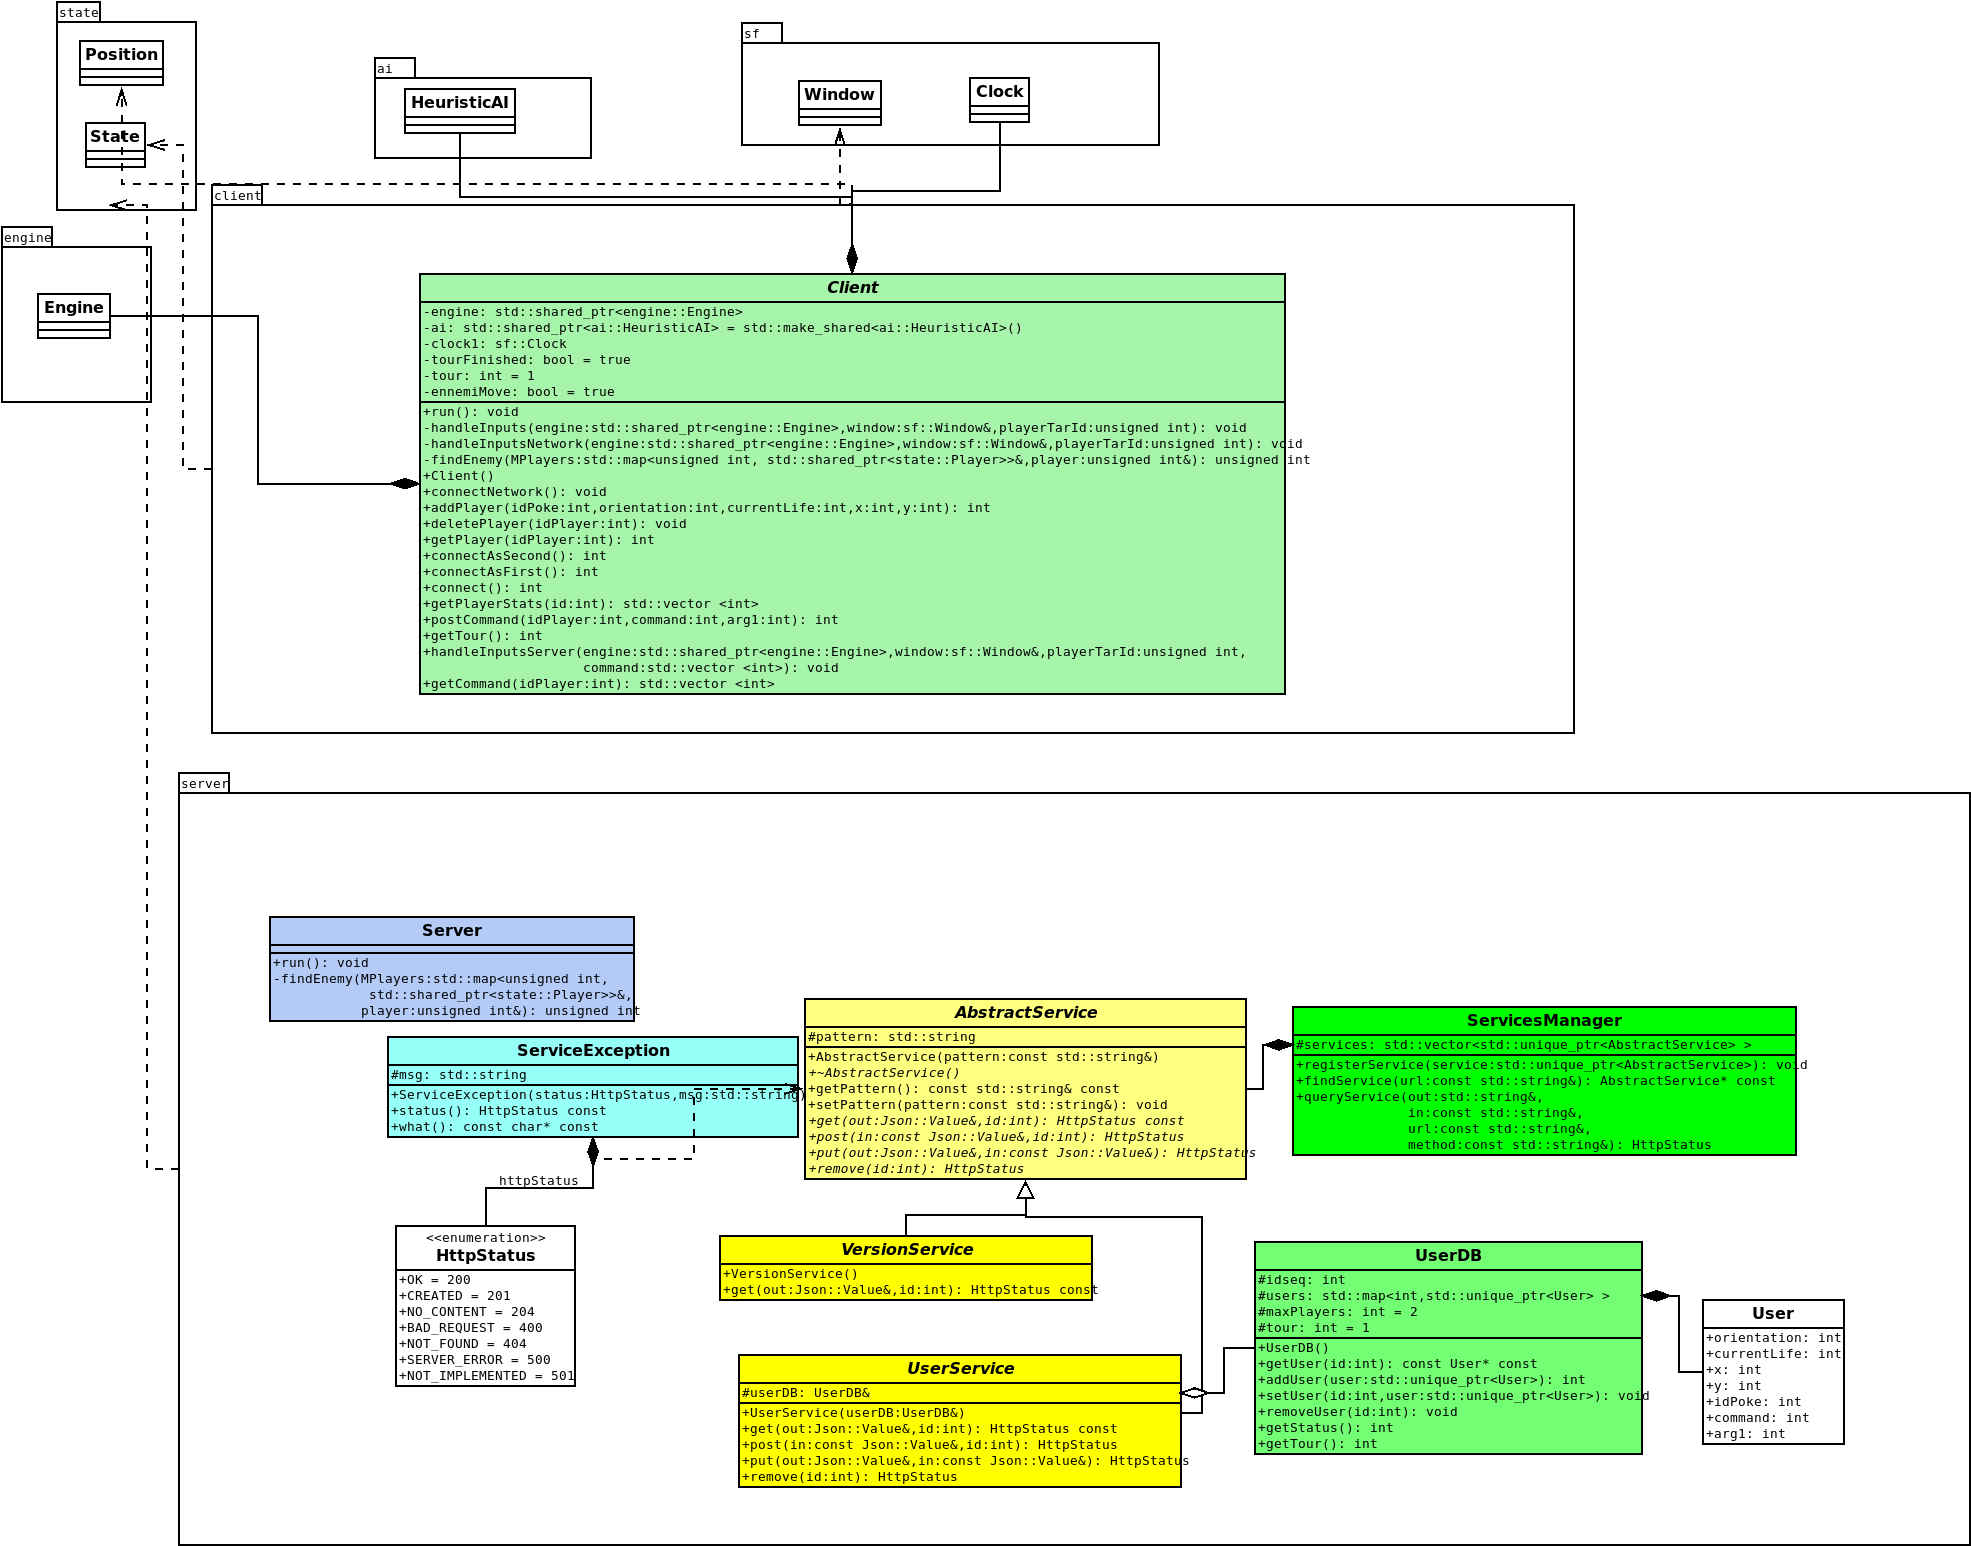
\includegraphics[width=0.9\paperheight]{module.png}
    \caption{\label{uml:module}Diagramme des classes pour la modularisation.}
    \end{figure}
    \end{landscape}
    
    \clearpage
    \section{Annexe}
    \label{sec:Annexe}
    \subsection{Bibliographie}

    


\end{document}
